\documentclass{ximera}

% vier voorkeuren die je meteen zelf kan instellen:
\def\uitbr{0} % waarde 1 als je Uitbreiding in de marge wilt, 0 als je dat niet wilt 
\def\wsg{0} % waarde 1 als je verwijzingen naar Wiskunde Samen gevat² in de marge wilt, 0 als je dat niet wilt
\def\rectoverso{0} % waarde 1 als je het PDF-bestand recto-verso wilt laten afdrukken, 0 als je het recto wilt
\def\voetn{1} % waarde 1 als je de voetnoten wilt, 0 als je dat niet wilt 

% marges:
\usepackage[paper=a4paper,margin=3.4cm,marginparwidth=2cm]{geometry}

% packages algemeen:
\pdfOnly{
\usepackage[english,dutch]{babel}
}
\usepackage{amsfonts}
\usepackage{amsmath} %  o.a. \eqref en \text, omgeving equation*
\usepackage{amssymb} % o.a. \nmid
\usepackage{amsthm} % o.a. omgeving proof
\usepackage{graphicx} % o.a. figuren
\usepackage{xcolor} % \color
\usepackage[disable]{todonotes} % \todo 
\usepackage{comment} % omgeving comment
\usepackage{xcolor} % kleuren 
\usepackage[skip=7pt plus1pt, indent=0pt]{parskip} % skip = verticale ruimte tussen twee alinea's, indent = insprong bij nieuwe alinea
\usepackage{multicol} % kolommen
\usepackage{xfrac} % breuken

\usepackage{siunitx} % SI eenheden
\usepackage{eso-pic} % achtergrond voorpagina
\usepackage{tabularx} % kolommen voor rekenmachine
\usepackage{rotating} % voor omgeving turn

% voor figuren met PSTricks:
\usepackage{pstricks} 
\usepackage{pstricks-add}
\usepackage{pst-plot}
\usepackage{pst-node}
\usepackage{pst-coil}
\usepackage{auto-pst-pdf}

% voor figuren met TikZ:
\usepackage{tikz} 
\usepackage{tkz-euclide} 
\usepackage{pgfplots} 
\usetikzlibrary{calc,intersections,through,backgrounds,patterns} 
\pgfplotsset{compat=newest}
\usepgfplotslibrary{fillbetween,colormaps}
\usepackage{import}
\usepackage{tikz-3dplot}

% zelfde parskip in minipage:
\makeatletter
\setlength{\parskip}{\medskipamount}
\newcommand{\@minipagerestore}{\setlength{\parskip}{\medskipamount}}
\makeatother

% voor veranderen van de naam Bibliografie naar Referentielijst:
\pdfOnly{
\addto\captionsdutch{\renewcommand{\bibname}{Referentielijst}}

% voor trefwoordenlijst:
\usepackage{imakeidx}
\makeindex[title=Trefwoordenlijst,program=makeindex,options=-s index.tex,columns=2,intoc=true]
}
% voor nummeren van vergelijkingen:
%WIM%\numberwithin{equation}{chapter} % als je dit desactiveert dan worden vergelijkingen in bijvoorbeeld hoofdstuk 3 genummerd als (1), (2) etc. in plaats van (3.1), (3.2) etc.

% voor hyperlinks en bladwijzers in PDF-bestand:
%WIM%\usepackage[bookmarksopen,bookmarksopenlevel=0,hypertexnames=false,pdfa,bookmarksnumbered]{hyperref} 
%WIM%\usepackage{bookmark} 

% voor hyperlinks: 
\hypersetup{pdfborder={0 0 0}, pdfstartpage=1,linkbordercolor={1 0 0}}%pdfborder={0 0 0} is geen rand rond hyperlinks, pdfborder={1 1 1} wel

% korter commando voor displaystyle, om bijvoorbeeld breuken groter te drukken in doorlopende tekst: 
\newcommand{\D}{\displaystyle}

% (veel)gebruikte verzamelingen:
\newcommand\NN{\mathbb{N}} % verzameling van de natuurlijke getallen
\newcommand\QQ{\mathbb{Q}} % verzameling van de rationale getallen
\newcommand\RR{\mathbb{R}} % verzameling van de re\"ele getallen
\newcommand\ZZ{\mathbb{Z}} % verzameling van de gehele getallen

% (veel)gebruikte operatoren:
\def\co{\operatorname{co}} % coördinaat van een punt
\def\ggd{\operatorname{ggd}} % positieve grootste gemene deler van twee gehele getallen niet beide nul
\def\gr{\operatorname{gr}} % graad van een veelterm

% voor kleur grafieken (donkergroen):
\definecolor{graf}{RGB}{0,100,0} 

% voor lijsten: 
% \usepackage{enumerate}
%WIM%\usepackage[shortlabels]{enumitem} 
\setlist{topsep=0em, itemsep=-0.15em}

% voor small bullet:
\newcommand\sbullet[1][.5]{\mathbin{\vcenter{\hbox{\scalebox{#1}{$\bullet$}}}}}

% voor meer verticale ruimte tussen vergelijkingen in align
\addtolength{\jot}{0.1cm}

% voor meervoudige voetnoten:
\usepackage{fnpct}

% voor het onderdrukken van voetnoten als optie:
\usepackage{letltxmacro}
\LetLtxMacro\Oldfootnote\footnote
\newcommand{\EnableFootNotes}{%
  \LetLtxMacro\footnote\Oldfootnote%
}
\newcommand{\DisableFootNotes}{%
  \renewcommand{\footnote}[2][]{\relax}
}

% voor verticale lijn in de marge (uitbreiding):
\usepackage[framemethod=default]{mdframed}
\usepackage{marginnote}
\reversemarginpar
\ifthenelse{\uitbr < 1}{\definecolor{rood}{RGB}{255,255,255}}{\definecolor{rood}{RGB}{254,64,64}} %HEX: #fe4040
\mdfdefinestyle{uitbreiding}{%
    topline=false,
    rightline=false,
    bottomline=false,
    leftline=true,
    linecolor=rood,
    linewidth=5pt,
    rightmargin=0pt,
    skipabove=10pt,% ipv 3
    skipbelow=0pt,
    leftmargin=-25pt,
    innerleftmargin=20pt,
    innerrightmargin=0pt,
    innertopmargin=0pt,
    innerbottommargin=0pt%,
%	needspace=30pt %minimumhoogte vooraleer lijn wordt gesplitst
    }
\newenvironment{Uitbreiding}{
    \marginpar{
        \center
		\vspace{0.1cm}
		\vspace{7pt}
		\rotatebox{90}{\color{rood}\Large \bf Uitbreiding}
	}
    \begin{mdframed}[style=uitbreiding]
    }{\vspace{-0.05cm}
    \end{mdframed}
}


% omgevingen voor lemma, definitie, voorbeeld etc.:
\newtheoremstyle{mystyle}
    {0em} % Space above
    {0em} % Space below
    {\itshape} % Body font
    {} % Indent amount
    {\bfseries} % Theorem head font
    {.} % Punctuation after theorem head
    {.5em} % Space after theorem head
    {} % Theorem head spec (can be left empty, meaning `normal')
\theoremstyle{mystyle}
%WIM%\newtheorem{lemma}{Lemma}[chapter] % als je [chapter] desactiveert dan Voorbeeld 3 in plaats van Voorbeeld 5.3, als je [chapter] vervangt door [section] dan Voorbeeld 5.2.3 in plaats van Voorbeeld 5.3 
%\theoremstyle{definition} % als je dit activeert dan is wat in de omgeving staat niet cursief gedrukt
\newtheorem{oefening}[lemma]{Oefening}
\newtheorem{definitie}[lemma]{Definitie} 
\newtheorem{voorbeeld}[lemma]{Voorbeeld}
\newtheorem{eigenschap}[lemma]{Eigenschap} 
\newtheorem{stelling}[lemma]{Stelling} 
\newtheorem{gevolg}[lemma]{Gevolg} 
\newtheorem{afspraak}[lemma]{Afspraak} 
\newtheorem{werkwijze}[lemma]{Werkwijze}

% omgeving proof, aangepaste ruimte: 
\makeatletter
\renewenvironment{proof}[1][\proofname]{\par
  \vspace{-\topsep}% remove the space after the theorem
  \pushQED{\qed}%
  \normalfont
  \topsep0pt \partopsep0pt % no space before
  \trivlist
  \item[\hskip\labelsep
        \itshape
    #1\@addpunct{.}]\ignorespaces
}{%
  \popQED\endtrivlist\@endpefalse
  \addvspace{0pt plus 0pt} % no space after
}
\makeatother

% kaderstijlen uit SOHO Wiskunde Plantyn:
\colorlet{steunkleur}{black}
\colorlet{steunkleurlicht}{steunkleur!30!white}
\colorlet{steunkleurkader}{steunkleur!7!white}
\colorlet{steunkleurkaderlicht}{steunkleur!2!white}

\mdfdefinestyle{kaderstijl_vol_licht}
{skipabove=6pt, 
skipbelow=6pt, 
backgroundcolor=steunkleurkader,
linecolor=steunkleurlicht,
linewidth = 0.4pt, 
topline=true,
bottomline=true, 
rightline=true,
innerleftmargin=5pt,
innerrightmargin=5pt,
innertopmargin=5pt,
leftmargin=0cm,
rightmargin=0cm,
innerbottommargin=5pt,
needspace=30pt % minimumhoogte voor splitsen kader
}
\surroundwithmdframed[style=kaderstijl_vol_licht]{definitie}
\surroundwithmdframed[style=kaderstijl_vol_licht]{stelling}
\surroundwithmdframed[style=kaderstijl_vol_licht]{lemma}
\surroundwithmdframed[style=kaderstijl_vol_licht]{eigenschap}
\surroundwithmdframed[style=kaderstijl_vol_licht]{gevolg}

% voor omgevingen voor oefening en antwoord:
\newenvironment{Oefening}{%
    \begin{enumerate}[ 
    series=Oef,
    resume=Oef,
    leftmargin=1.78em,
    label={\bfseries\arabic*.},
    ref=\arabic*
    ]
    \item %
    }{%
    \end{enumerate}
}
\newenvironment{Antwoord}{%
    \begin{enumerate}[%
    series=Antw,
    resume=Antw,
    leftmargin=1.78em,
    label={\bfseries\arabic*.},
    ref=\arabic*
    ]
    \item %
    }{%
    \end{enumerate}
}

% als de omgeving Uitbreiding start met een kaderomgeving (definitie, stelling, eigenschap, lemma of gevolg) dan moet wat extra verticale ruimte voorzien worden, met het commando \uitbreidingstartmetkader:
\def\uitbreidingstartmetkader{\mbox{}\vspace{-0.205cm}}

% % voor schema van de staartdeling:
% \usepackage{stackengine}
% \setstackgap{S}{5pt}
% \stackMath\def\stackalignment{r}
% \newcommand{\myRule}[3][white]{\textcolor{#1}{\rule{#2}{#3}}}
% \let\ph\phantom % enkel voor tekst
% \newcommand{\mph}[1]{% enkel voor math mode
%     \mathcolor{white}{#1}%
% }
% \def\staartmin{\rule{0.25cm}{0.1mm}\myRule{0.3cm}{0.1mm}}
% \def\staartphmin{\myRule{0.25cm}{0.1mm}\myRule{0.3cm}{0.1mm}}
% \newcommand{\staartstreep}[1]{\rule{\widthof{$#1$}}{0.1mm}}
% \newcommand{\staartphstreep}[1]{\myRule{\widthof{$#1$}}{0.1mm}}

% voor kolommen met schema van Horner:
\newcommand{\kolbreed}{1.0cm}
\newcolumntype{H}{>{\centering\arraybackslash$} p{\kolbreed} <{$}}

% voor nieuw commando utikzdashed: onderlijn (zoals underline) maar dan met stippellijn:
\tikzset{
    cheating dash/.code args={on #1 off #2 ends #3}{%
        \csname tikz@addoption\endcsname{%
            \pgfgetpath\currentpath%
            \pgfprocessround{\currentpath}{\currentpath}%
            \csname pgf@decorate@parsesoftpath\endcsname{\currentpath}{\currentpath}%
            \pgfmathparse{max(#1-#3,0)}\let\dashphase=\pgfmathresult%
            \pgfmathparse{\csname pgf@decorate@totalpathlength\endcsname-#1+2*\dashphase}\let\rest=\pgfmathresult%
            \pgfmathparse{#1+#2}\let\onoff=\pgfmathresult%
            \pgfmathparse{max(floor(\rest/\onoff), 1)}\let\nfullonoff=\pgfmathresult%
            \pgfmathparse{max((\rest-\onoff*\nfullonoff)/\nfullonoff+#2, #2)}\let\offexpand=\pgfmathresult%
            \pgfsetdash{{#1}{\offexpand}}{\dashphase pt}}%
    },
    cheating dash per segment/.style args={on #1 off #2 ends #3}{
        /utils/exec=\csname tikz@options\endcsname,%
        decoration={show path construction,
            lineto code={\draw [cheating dash=on #1 off #2 ends #3] (\tikzinputsegmentfirst) -- (\tikzinputsegmentlast);},
            curveto code={\draw [cheating dash=on #1 off #2 ends #3] (\tikzinputsegmentfirst) .. controls (\tikzinputsegmentsupporta) and (\tikzinputsegmentsupportb) .. (\tikzinputsegmentlast);},
            closepath code={\draw [cheating dash=on #1 off #2 ends #3] (\tikzinputsegmentfirst) -- (\tikzinputsegmentlast);}
        },
        decorate,
    },
}
\newcommand{\utikzdash}[1]{%
    \tikz[baseline=(todotted.base)]{
        \node[inner sep=0pt,outer sep=1.5pt] (todotted) {#1};
        \draw[cheating dash per segment=on 2pt off 2pt ends 2pt, line width=0.4pt] (todotted.south west) -- (todotted.south east);
    }%
}%

\providecommand{\xmemph}[1]{\textit{#1}}

% voor nieuw commando underdashed: onderlijn met stippellijnen en ook het woord cursief zetten:
\newcommand{\underdashed}[1]{%
    {\em\utikzdash{\!#1\!}}%
}

% voor icoon TI-84 Plus met verwijzing naar filmpje:
\newcommand{\grmlink}{\raisebox{0cm}{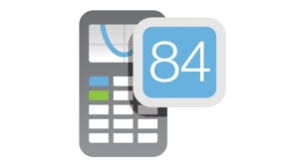
\includegraphics[width=1cm]{TI84Plus-icoon}}}
\newcommand{\grmref}[1]{%
	\reversemarginpar%
	\marginpar{
		\vspace{-0.4cm}%
		\htmladdnormallink{\grmlink}{#1}
	}	
}

% GRM knoppen:
\newcommand{\GRM}[1]{\fbox{\rule[0mm]{0cm}{0.215cm}\textup{\texttt{#1}}}}
\newcommand{\wedgetext}{{\raisebox{0.02cm}{\begin{turn}{90}>\end{turn}}}}
\newcommand{\veetext}{\raisebox{0.2cm}{\begin{turn}{-90}>\end{turn}}}

% voor kolommen met GRM screens:
\newlength{\widthallscreens}
\newlength{\widthscreens}
\newlength{\spaceleftscreen}
\newlength{\spacerightscreen}
\newlength{\spacebetweenscreens}

\newcommand{\setscreens}{
	\setlength{\spaceleftscreen}{2pt}
	\setlength{\spacerightscreen}{2pt}
	\setlength{\spacebetweenscreens}{8pt}
	\addtolength{\linewidth}{-28pt} % 3*8pt tussen vier screens en 2 pt links en 2 pt rechts
	\setlength{\widthallscreens}{\linewidth}
	\setlength{\widthscreens}{0.25\widthallscreens}
	\addtolength{\linewidth}{28pt}
	\newcolumntype{G}{p{\widthscreens}}
	\newcolumntype{s}{p{\spacebetweenscreens}}
	\newcolumntype{L}{p{\spaceleftscreen}}
	\newcolumntype{R}{p{\spacerightscreen}}
	\setlength{\tabcolsep}{0pt}
}

% voor icoon met verwijzing naar Wiskunde Samen gevat² in de marge:
% \newcommand{\wsglink}{\raisebox{0cm}{\includegraphics[width=1cm]{wsglogo}}}
\newcommand{\wsglink}{\raisebox{0cm}{LOGO}}
\newcommand{\htmladdnormallink}[2]{\href{#2}{#1}}
\newcounter{pagnrwsg}
\newcommand{\wsgref}[3]{% 
    % #1 woord dat onderstippeld wordt
    % #2 pagina van Wiskunde Samen gevat² waar je op terecht komt als je op de link klikt  
    % #3 afgedrukt op het logo van Wiskunde Samen gevat² in de marge: één of meerdere paginanummers
    \ifthenelse{\wsg < 1}{#1}{%
        \underdashed{#1}%
        {\setcounter{pagnrwsg}{#2}}%
        {\addtocounter{pagnrwsg}{14}}%
        \reversemarginpar%
        \marginpar{\vspace{-0.6cm}%
           \htmladdnormallink{\wsglink}{https://online.fliphtml5.com/sanky/laea/\#p=\arabic{pagnrwsg}}%
            \raisebox{0.41cm}[0cm][0cm]{%
                \hspace{-1.5cm}\makebox[2cm][c]{\colorbox{white}{\texttt{\footnotesize{#3}}}}%
            }%
        }%
    }%
}

% voor invoegen blanco pagina bij de optie recto-verso:
\def\blancobijrectoverso{
	\ifthenelse{\rectoverso < 1}{\clearpage}{
	\clearpage
	\thispagestyle{empty}
	\mbox{}
	\clearpage
	}
}

% aantal pagina's van het bestand:
\ifthenelse{\rectoverso < 1}{\def\totpag{57}}{\def\totpag{66}}

% documenteigenschappen:
% \usepackage{hyperxmp}
% \hypersetup{
% pdftitle={Open Source Wiskunde Aan zet: Veeltermen}, 
% pdfnumpages={\totpag},
% pdfauthor={Koen De Naeghel},
% pdflang={nl},
% pdfkeywords={wiskunde, open source, wiskunde aan zet, veeltermen, secundair onderwijs, tweede graad, doorstroomfinaliteit},
% pdfsubject={Veeltermen},
% pdfcopyright={\unichar{"24B8} 2024 Koen De Naeghel},
% pdfdate={17 december 2024},
% pdfapart=1,
% pdfstartview=}

% voor het benoemen van titel, auteur en datum:
% \title{Veeltermen}
% \author{Auteur: Koen De Naeghel}
% \date{\today}

\newcommand\BackgroundPic{
    \put(-260,-125){
    \parbox[b][\paperheight]{\paperwidth}{%
    \vfill
    \centering
    
\includegraphics[height=\paperwidth, keepaspectratio]{WaZlogo}%
    \vfill
}}}

\addPrintStyle{..}
\begin{document}
    \author{Wiskunde Op Maat }
    \xmtitle{De goniometrische schrijfwijze van complexe getallen}{}
     
    \label{xim:complexe_getallen_polair}  % goniometrisch ???
 



In het vorig hoofdstuk werk een punt in het complexe vlak beschreven met carthesische coordinaten. Op die manier werd elk complex getal weergegeven in de carthesische vorm $z=a+bi$. In dit hoofdstuk wordt een alternatieve manier behandeld om punten in het complexe vlak te beschrijven. Hiermee zullen verschillende operaties van complexe getallen, waaronder de vermenigvuldig, veel eenvoudiger en inzichtelijker worden. 

\begin{quickquestion*}{}
    Is er een andere manier waarmee je een punt in het vlak zou kunnen beschrijven? 
\end{quickquestion*}




 
%complexe getallen in Polaire vorm 

De carthesische schrijfwijze associeert met een elk complex getal $z=a+bi$ het koppel \((a, b)\). Het reeël deel \(a\) komt overeen met de projectie op de reële as, het imaginair deel \(b\) komt overeen met de projectie op de imaginaire as. De polaire vorm associeert met elk complex getal in het vlak een koppel poolcoördinaten \((r, \theta)\).  Hierbij is $r=|z|$ de norm (afstand tot de oorsprong) en $\theta$, de hoek die de overeenkomstige vector maakt met de positieve reële as. Op die manier wordt elk complex getal beschreven met een uniek koppel poolcoordinaten. 


\begin{definition}
    Het koppel $(r,\theta)$ zijn de \textit{poolcoördinaten} van het punt $z$. We noemen $r=|z|$ de \textbf{modulus} en $\theta$ het \textbf{argument}. De hoek $\theta$ wordt gemeten in radialen, in tegenwijzerzin, en is slechts op een veelvoud van $2\pi$ na bepaald.
\end{definition}


 
% AAN AFBEELDINGEN WERKEN; DE CARTHESISCHE VOOR DE DEFNITIE; POLAIR IN DE DEFINITIE 
 
 \begin{image}%[\textwidth]
    \begin{tikzpicture}[scale=5]%,cap=round,transform canvas={scale=0.5}]
     
    \tikzmath{\hoek = 30; \myc = cos(\hoek); \mys = sin(\hoek);
        \hoekb = 20;}
     
    % Goniometrische cirkel
    %   \draw (0,0) circle (1cm);
    \draw[->] (-0.1,0) -- (1.3,0) node[above] {Re$(z)$};
    \draw[->] (0,-0.1) -- (0,0.9) node[below right] {Im$(z)$};
     
    \draw[color=blue,thick] (0:0)  -- node[right] {\small$r=|z|=\sqrt{a^2+b^2}$} (\hoek:1);
    %
    \draw[color=black] (\hoek:1) node[name=P,circle, fill=black, radius=1pt,scale=0.8] {} node [yshift=1pt,above,align=center] {$z=a+bi$\\$=r(\cos\theta+i\sin\theta)$} ; 
    %
    \draw[dashed] ({cos(\hoek)},0) node[circle, fill=black, radius=1pt,scale=0.5] {} node[below] {\color{red}$a=r\cos\theta$} -- (P);
    \draw[dashed] (0,{sin(\hoek)}) node[circle, fill=black, radius=1pt,scale=0.5] {} node[left] {\color{red}$b=r\sin\theta$} -- (P);
    \draw[color=blue, ->] (0.3,0) arc (0:\hoek:0.3cm) node [midway,right] {$\theta$ met $\tan\theta = \frac ba$};  
     
    \end{tikzpicture}
\end{image}


 
 
%Indien $z=0$, stellen we per conventie $\theta=0+2k\pi, \; \mbox{met } k\in \Z$.
%\\ De hoek $\theta$ voor een gegeven $z$ is niet uniek bepaald.
%Wanneer we bij $\theta$ een geheel veelvoud van $2\pi$ bijtellen
%vinden we hetzelfde punt en dus hetzelfde complex getal terug.
 
% Er wordt niet gezegd wat r en theta zijn in deze definitie.
%\begin{definition}
%Een \textbf{goniometrische} (ook \textbf{polaire}) \textbf{voorstelling} van een complex getal $z = a+bi\in\C$ is
%$$
%\important{z = r(\cos\theta+i\sin\theta)}.
%$$
%waarbij de sinus en cosinus \textit{niet} worden uitgerekend.
%
%Hierbij is $r=|z|$ de \textbf{modulus} en $\theta$ het \textbf{argument} (ook \textbf{fase}).
%\end{definition}
 
 % Merk dus op dat aan de hand van de modulus $r$ en het argument $\theta$ van een complex getal $z$, het reële deel van $z$ gelijk is aan $a = r\cos \theta$, en het imaginaire deel gelijk is aan $b = r\sin \theta$.
 
%Men noteert dit soms ook als $r\angle \theta$.\\
 

 
 
Men kan een complexe getal in carthesische schrijfwijze $z=a+bi$ omvormen naar polaire vorm $z = r(\cos \theta + i\sin\theta)$ en vice versa. Het zal blijken dat sommige berekeningen veel eenvoudiger zijn in één van beide schrijfwijzes. De stelling van pythagoras en de goniometrische getallen leggen het verband tussen de carthesische en polaire schrijfwijze. 

\begin{proposition}[Transformatieformules cartesische en goniometrische  schrijfwijze]\label{eig:transformatie_complexe_getallen} \nl
     
    Een complex getal $z$ met goniometrische schrijfwijze $r(\cos \theta + i\sin\theta)$ heeft als cartesische schrijfwijze $a+bi$ met:
    \begin{center}
        \important{a =  r \cos \theta}\\
        \important{b =  r \sin \theta}
    \end{center}
    Een complex getal $z$ met cartesische schrijfwijze $a+bi$ heeft als goniometrische schrijfwijze $r(\cos \theta + i\sin\theta)$ met:
    \begin{align*}
    \important{r = \sqrt{a^2+b^2}} \\
    \important{\cos\theta  = \dfrac{a}{\sqrt{a^2+b^2}}}\\
    \important{\sin\theta  = \dfrac{b}{\sqrt{a^2+b^2}}}
    \end{align*}
\end{proposition}

 
\begin{remark}\nl
     
    \begin{itemize}
        \item Omdat $\theta$ niet uniek bepaald is, heeft elk complex getal $z = r(\cos\theta+i\sin\theta)$ \textit{oneindig veel goniometrische schrijfwijzes} $z = r\left(\cos(\theta+k2\pi)+i\sin(\theta+k2\pi) \right)$, met $k\in\Z$. Vaak wordt er echter voor gekozen om $\theta$ tussen 0 en $2\pi$ te geven: we kunnen ons sneller voorstellen waar de hoek $\frac{5\pi}{4}$ ligt dan de hoek $\frac{1093\pi}{4}$.
        \item Twee complexe getallen in goniometrische schrijfwijze zijn gelijk aan elkaar als ze dezelfde modulus hebben, en hun argument gelijk is op een veelvoud van $2\pi$ na.
        %$$
        %r_1(\cos\theta_1+i\sin\theta_1)=r_2(\cos\theta_2+i\sin\theta_2)\quad\Leftrightarrow
        %\quad r_1=r_2 \; \mbox{ en }\; \exists k\in \Z:\theta_1=\theta_2+2k\pi.
        %$$
    \end{itemize}
     
\end{remark}
 
\begin{exercise}\nl
    Geef de goniometrische schrijfwijze van volgende complexe getallen waarvan het argument gemakkelijk grafisch gevonden kan worden:
    \begin{question} $z=1 $
        \begin{oplossing}
          Voor $z=1 $ is de modulus $1$ en het argument $0$, dus de goniometrische schrijfwijze is $$z= \cos 0 + i\sin 0 \text{  of  } z= \cos 2\pi + i\sin 2\pi.$$
        \end{oplossing}
    \end{question}
\begin{question} $z=i $
    \begin{oplossing}
     Voor $z=i $ is de modulus $1$ en het argument $\frac{\pi}{2}$, dus de goniometrische schrijfwijze is $$z= \cos\frac{\pi}{2} + i \sin \frac{\pi}{2}.$$  
    \end{oplossing}
\end{question}
    \begin{question} $z=1+i$
        \begin{oplossing}
            Voor $z=1+i$ is de modulus $\sqrt{2}$ en het argument $\frac{\pi}{4}$, dus de goniometrische schrijfwijze is $$z= \sqrt{2}(\cos \frac{\pi}{4}+i\sin\frac{\pi}{4}).$$ 
        \end{oplossing}
    \end{question}
    \begin{question} $z=\frac{\sqrt2}{2}+i\frac{\sqrt2}{2}$
        \begin{oplossing}
            Voor $z=\frac{\sqrt2}{2}+i\frac{\sqrt2}{2}$ is de modulus $1$ en het argument $\frac{\pi}{4}$, dus de goniometrische schrijfwijze is $$z = \cos \frac{\pi}{4}+i\sin\frac{\pi}{4}.$$
        \end{oplossing}
    \end{question}
     
    Merk op: bij het opschrijven van de goniometrische schrijfwijze met concrete getallen moet je de $\sin$ en $\cos$ laten staan. Als je die toch zou uitrekenen, krijg je immers terug de cartesische schrijfwijze.
\end{exercise}
 


 
\begin{basicSkip}
Je kan verder experimenteren met volgende applet: Je kan $z= a+bi=r(\cos \theta+ i  \sin \theta)$ verplaatsen en telkens $a=\text{Re}(z)$, $b=\text{Im}(z)$, $r=|z|$ en $\theta$ aflezen.
 
\geogebra{NwzgUCQG}{887}{528}
\end{basicSkip}
 
 
 
 

 
 
\begin{remark}\nl
     
    Als $a \neq 0$ kunnen we de tweede vergelijking delen door de eerste (waardoor de vierkantswortel wegvalt) en krijgen we
    $$
    \tan \theta = \frac{b}{a}  \quad \text{ als } a \neq 0
    $$
    Als $a >0$ dan is $\theta$ een hoek in het 1ste of het 4de kwadrant en is dus per definitie van de \hyperref[xim:cyclometrische_functies]{boogtangens }
    $$
    \theta  =  \bgtan \left(\frac{b}{a}\right) \quad \text{ als }  a>0
    $$
    Als $a<0$ dan is $\theta$ een hoek in het 2de of het 3de kwadrant en dan geldt
    $$
    \theta  =  \bgtan \left(\frac{b}{a}\right) + \pi \quad \text{ als }  a<0
    $$
    Als $a=0$, dan ligt $z=a+bi$ op de $y$-as en geldt
    \begin{align*}
    \theta & =  \frac{\pi}{2}  \quad\text{ als } a=0, b > 0\\
    \theta & = -\frac{\pi}{2} \quad\text{ als } a=0, b < 0
    \end{align*}
     
    Samengevat geeft dit voor $\theta$:
    $$
    \theta = \begin{cases}
    \bgtan \frac{b}{a}       & \text{ als } a>0        \\
    \pi + \bgtan \frac{b}{a} & \text{ als } a<0        \\   % met \pi+... lopen de breuken elkaar minder in de weg dan met ...+pi!
    \frac{\pi}{2}            & \text{ als } a=0, b > 0 \\
    -\frac{\pi}{2}           & \text{ als } a=0, b < 0
    \end{cases}
    $$
    \begin{basicSkip}
Dit alles wordt ook uitgelegd in onderstaande video:
 
\youtube{_qLKTopxSXc}
\end{basicSkip}
 
\end{remark}
% Bron: SPOC Complexe Getallen https://tube.geogebra.org/material/iframe/id/NwzgUCQG/width/887/height/528/border/888888/rc/false/ai/false/sdz/false/smb/false/stb/false/stbh/true/ld/false/sri/false/at/auto
 
 
 
\xmsection{Vermenigvuldiging van complexe getallen in goniometrische schrijfwijze}\nl
 
In de goniometrische schrijfwijze is het niet eenvoudig om complexe getallen op te tellen: hiervoor is de cartesische schrijfwijze veel makkelijker, omdat we dan gewoon reëel en imaginair deel bij elkaar moeten optellen. Voor de vermenigvuldiging van complexe getallen is het andersom: daarvoor is er de volgende interessante formule voor de goniometrische schrijfwijze:
 
Als $z_1=r_1 (\cos \theta_1 + i \sin \theta_1 ) $ en $z_2 = r_2(\cos \theta_2 + i \sin \theta_2 )$ twee complexe getallen zijn, dan is
\begin{align*}
z_1\cdot z_2 &= r_1 (\cos \theta_1 + i \sin \theta_1 )\cdot r_2 (\cos\theta_2 + i \sin \theta_2 )\\
             &= r_1 r_2 (\cos \theta_1 \cos \theta_2 - \sin \theta_1  \sin\theta_2 + i(\sin \theta_1 \cos \theta_2 + \cos \theta_1  \sin
\theta_2 ))\\
             &= r_1 r_2 ( \cos(\theta_1 + \theta_2) + i \sin(\theta_1 + \theta_2)) \, ,
\end{align*}
waarbij we in de laatste stap gebruik hebben gemaakt van de \hyperref[xim:goniometrie_formules]{som- en verschilformules}.
Dit betekent dat de moduli $r_i$ moeten worden vermenigvuldigd, en de argumenten $\theta_i$ moeten worden opgeteld.
 
\begin{proposition}[Vermenigvuldiging van twee complexe getallen in goniometrische schrijfwijze]\label{eig:vermenigvuldiging_complexe_getallen}\nl
     
De \textit{modulus} van het product van twee complexe getallen is het \textit{product van de moduli} van die getallen.
 
Het \textit{argument} van het product van twee complexe getallen is de \textit{som van de argumenten} van die getallen.
\end{proposition}
 
\begin{xmuitweiding}[Vermenigvuldiging van 2 complexe getallen grafisch uitgelegd]
We kunnen de vermenigvuldiging met een complex getal ook zien als een soort van actie die we doen op punten in het vlak. Als we een bepaald complex getal $z = r(\cos\theta + i \sin \theta)$ fixeren, en eender welk complex getal vermenigvuldigen met die $z$, dan tellen we steeds $\theta$ bij het argument van het complex getal op, en vermenigvuldigen we de modulus van dat complex getal steeds met $r$.
 
% Als je focust op het effect van vermenigvuldiging met één complex getal, krijg je %%% vind ik precies wat een vreemde zin?
\begin{proposition}[Vermenigvuldiging met een complex getal in goniometrische schrijfwijze $z=r(\cos\theta + i\sin\theta)$]\nl
     
Vermenigvuldigen met $z = r(\cos\theta + i\sin\theta)$ betekent \textit{roteren} over een hoek $\theta$ en afstanden en lengtes \textit{herschalen} met een factor $r$.
\end{proposition}
 
Je kan experimenteren met deze voorstelling van de vermenigvuldiging door in onderstaande applet de complexe getallen $z_1$ en $z_2$ te verslepen, en dan via de vermenigvuldig-knop te zien hoe vermenigvuldigen met $z_2 = (r,\theta)$ inderdaad kan beschouwd worden als een \textit{rotatie} over een hoek $\theta$ gevolgd door een \textit{herschaling} met een factor $r$.
 
\geogebra{i0Lbx90s}{893}{451}
\end{xmuitweiding}
 
\begin{xmuitweiding}[Inverse van een complex getal met poolcoördinaten]
We zijn geïnteresseerd in het volgende probleem: stel dat je een complex getal $z$ hebt, met welk ander complex getal, zeg $w$, moet je $z$ vermenigvuldigen zodat het resultaat 1 geeft? Met andere woorden: hoe bepaal je de \textit{inverse} van een complex getal?
 
Stel dat het complex getal $z$ zuiver reëel is, dus zodanig dat de cartesische schrijfwijze van $z$ van de vorm $z = a + 0i$ is. Dan is het makkelijk om te vinden wat de inverse is: door te vermenigvuldigen met $w = 1/a$ komen we op 1 uit. Het algemene geval is echter lastiger met cartesische coordinaten,
% als $z = a + bi$, en $w = c + di$, dan wordt de vergelijking $z\cdot w = 1$:
%$$
%z\cdot w = (a+bi)\cdot (c+di) = (ac -  bd) + (bc + ad)i = 1 + 0i \, .
%$$
%Dit komt neer op een stelsel van twee vergelijkingen in twee onbekenden:
%$$
%\begin{cases}
%ac - bd &= 1 \\
%bc + ad &= 0
%\end{cases}
%$$
maar zal makkelijker zijn met poolcoördinaten, aangezien het hier gaat over vermenigvuldigingen van complexe getallen. Als we de rekenregels voor het vermenigvuldigen van complexe getallen in goniometrische schrijfwijze in het achterhoofd houden, vinden we het volgende:
 
\begin{proposition}
Stel dat het complexe getal $z$ modulus $r$ en argument $\theta$ heeft. Dan is de inverse van $z$ het complexe getal met modulus $1/r$ en argument $-\theta$. 
\end{proposition}
 
Uiteraard bestaat de inverse dus niet voor het complex getal nul. Voor $z\neq 0$, met $(r, \theta)$ als poolcoördinaten, is de inverse inderdaad het complex getal $w$ met poolcoördinaten $\left(\frac{1}{r}, -\theta\right)$: de modulus van het product van complexe getallen is het product van de moduli, terwijl het argument van het product van complexe getallen de som van de argumenten is. Dus $z\cdot w$ heeft modulus 1, en argument 0: dit zijn precies de poolcoördinaten van het getal 1.
\end{xmuitweiding}
 
%Indien de cartesiaanse vorm gegeven is, kan de modulus bepaald worden met de stelling van Pythagoras, en de hoek $\theta$ in de rechthoekige driehoek met rechthoekszijden $|a|$ en $|b|$. Merk op dat voor $a<0$, het complex getal in het tweede of derde kwadrant ligt. 
%Aangezien $\arctan$ per definitie steeds als resultaat een hoek in het interval $]-\pi/2,\pi/2[$ geeft, dient  in de uitdrukking voor het argument $\theta$ een term $\pi$ toegevoegd te worden om correct te zijn.
%Als $|a|$ of $|b|$ gelijk is aan 0, redeneer je niet in een driehoek, maar ligt het complex getal op \'e\'en van de assen en kan je het argument $\theta$ onmiddellijk aflezen op een figuur.
 
 
% verdere inhoud over complexe getallen uit Zomercursus 201x in kwadratische_vergelijking/veeltermen/...
 
%\begin{thebibliography}{9}
%\bibitem{nieuwe delta} P. Gevers, J. Anseeuw, J. De Langhe, G. Roels, H. Vercauter,
%\textit{Nieuwe Delta, 5/6 Complexe Getallen(6 - 8 uur)}, Leuven,
%Wolters Plantyn, 1994.
%\bibitem{Jennekens}E. Jennekens, G. Deen, \textit{Wiskunde '68, Wiskunde 5, Deel A, Matrices en
%complexe getallen}, Antwerpen, De Sikkel, 1972.
%\bibitem{Quaegebeur}
%J. Quaegebeur, \textit{Basisbegrippen en basistechnieken uit de
%wiskunde}, Leuven, Acco, 2004.
%\bibitem{Croft}A. Croft and R. Davison, \textit{Mathematics for engineers}, Pearson Education Limited, third edition, 2008.
%\end{thebibliography}
%
%\newpage
 
\end{document}